% omega_m binning -- status slides (October 2026)
% Compile: pdflatex omega_m_binning.tex (twice). Figures in figs/ (PDF), made by the scripts in scripts/.
\documentclass[aspectratio=169,10pt]{beamer}
\usepackage[T1]{fontenc}
\IfFileExists{lmodern.sty}{\usepackage{lmodern}}{}
\usepackage{amsmath,amssymb}
\usepackage{booktabs}
\usepackage{graphicx}
\usepackage{xcolor}
\usepackage{array}
\graphicspath{{figs/}}

% ---------------------------------------------------------------- look
\definecolor{ink}{HTML}{1A1A19}
\definecolor{muted}{HTML}{6B6A63}
\definecolor{accent}{HTML}{2A78D6}
\definecolor{one}{HTML}{EB6834}
\definecolor{two}{HTML}{2A78D6}
\definecolor{three}{HTML}{1BAF7A}
\definecolor{wash}{HTML}{EEF4FC}
\setbeamercolor{normal text}{fg=ink}
\setbeamercolor{frametitle}{fg=ink}
\setbeamercolor{title}{fg=ink}
\setbeamercolor{structure}{fg=accent}
\setbeamercolor{itemize item}{fg=accent}
\setbeamercolor{itemize subitem}{fg=muted}
\setbeamerfont{frametitle}{size=\large,series=\bfseries}
\setbeamertemplate{navigation symbols}{}
\setbeamertemplate{itemize items}[circle]
\setbeamertemplate{frametitle}{%
  \vspace*{0.35em}\insertframetitle\par\vspace{-0.2em}%
  {\color{accent}\rule{\textwidth}{0.6pt}}\vspace{-0.6em}}
\setbeamertemplate{footline}{%
  \hspace*{0.6em}{\color{muted}\scriptsize $\omega_m$ binning --- status, October 2026}\hfill
  {\color{muted}\scriptsize\insertframenumber}\hspace*{0.8em}\vspace*{0.45em}}
\setlength{\leftmargini}{1.1em}
\setlength{\leftmarginii}{1.0em}
\newcommand{\takeaway}[1]{%
  \begin{beamercolorbox}[wd=\textwidth,sep=0.45em]{}\colorbox{wash}{\parbox{\dimexpr\textwidth-2\fboxsep}{\small #1}}\end{beamercolorbox}}
\newcommand{\om}{\omega_m}
\newcommand{\lcdm}{$\Lambda$CDM}
\newcommand{\sm}{\scriptsize}

\title{Freeing $\omega_m$ across multipoles}
\subtitle{A CMB diagnostic of \lcdm: model, binning, mock-data MCMC and code benchmarks}
\author{Marco Bella}
\institute{Knox Research Group, UC Davis}
\date{October 2026}

\begin{document}

% ======================================================================
\begin{frame}[plain]
  \vfill
  {\color{ink}\LARGE\bfseries Freeing $\omega_m$ across multipoles\par}
  \vspace{0.4em}
  {\color{muted}\large A CMB diagnostic of \lcdm: model, binning, mock-data MCMC and code benchmarks\par}
  \vspace{0.8em}{\color{accent}\rule{0.6\textwidth}{0.8pt}}\par\vspace{0.8em}
  Marco Bella \quad {\color{muted}Knox Research Group, UC Davis}\par
  {\color{muted}October 2026}
  \vfill
  {\color{muted}\scriptsize All results use mock (noiseless) Planck-like data. Chains: 8 $\times$ $10^5$ steps per run on Hive.}
\end{frame}

% ======================================================================
\begin{frame}{The idea: let $\omega_m$ depend on the multipole}
\begin{columns}[T]
\column{0.55\textwidth}
\begin{itemize}
  \item Split $\ell = 2\ldots2508$ into $N$ bins; bin 0 $=[2,\ell_{s,1}]$, bin $i=(\ell_{s,i},\ell_{s,i+1}]$.
  \item In bin $i$ every spectrum (TT, TE, EE, $\phi\phi$) is the \lcdm\ one with
  \[ \omega_{\rm cdm} = \omega_{m,i}-\omega_b , \]
  all other parameters ($\omega_b, h, \tau, n_s, A_s$) shared.
  \item \lcdm\ $\Leftrightarrow$ $\omega_{m,0}=\dots=\omega_{m,N-1}$.\\
  Test: $\chi^2 = \bar\Delta^{T} C_\Delta^{-1}\bar\Delta$ on $\Delta_i=\omega_{m,i}-\omega_{m,0}$, $N-1$ d.o.f.
  \item The bin edges $\ell_{s,i}$ are fixed in each run (not sampled).
\end{itemize}
\column{0.43\textwidth}
\begin{itemize}
  \item[] {\bfseries What it is}: a scale-dependent consistency test. Physics that changes the damping tail differently from the
  acoustic peaks shows up as $\omega_{m,i}\neq\omega_{m,j}$.
  \item[] {\bfseries What it is not}: a cosmology. There is no single background, so $\Omega_m$, $H(z)$, $\sigma_8$, $r_s$ are undefined
  $\Rightarrow$ CMB-only, no BAO/SN.
  \item[] {\bfseries By construction}: spectra jump at the bin edges (slide~\ref{fr:edges}).
\end{itemize}
\end{columns}
\vspace{0.6em}
\takeaway{Three questions for this talk: (1) where to put the edges, (2) does the binned fit detect a step it was not designed for,
and (3) can we trust the fast spectra (CosmoPower) we use for the chains?}
\end{frame}

% ======================================================================
\begin{frame}{Pipeline}
\begin{columns}[T]
\column{0.5\textwidth}
{\bfseries Sampler}: MontePython 3.6.1 (Metropolis--Hastings), shared by both pipelines.
\begin{itemize}\small
  \item 8 chains $\times\ 10^5$ steps per run, 30\% burn-in.
  \item Proposal: inverse Fisher matrix of the same likelihood.
  \item Convergence: $R-1 \le 0.002$ for every parameter of every run; acceptance 0.14--0.30.
\end{itemize}
\vspace{0.4em}
{\bfseries Parameters}: $100\,\omega_b, h, \tau_{\rm reio}, n_s, \ln(10^{10}A_s)$, $\omega_{m,0..N-1}$; flat priors
($h\in[0.6,0.75]$, $\omega_{m,i}\in[0.05,0.25]$).
\column{0.48\textwidth}
{\bfseries Two spectra back-ends, same interface} (a \texttt{classy} look-alike, so MontePython is unchanged):
\vspace{0.3em}
\begin{center}\small
\begin{tabular}{@{}p{0.27\linewidth}p{0.69\linewidth}@{}}
\toprule
\texttt{with\_}\newline\texttt{cosmopower} & CosmoPower CP\_paper emulators (TT, EE, TE, $\phi\phi$; lensed; $\ell\le2508$), one batched call per bin. $\sim$0.1 s/step. \\
\addlinespace
\texttt{with\_class} & real CLASS v3.4, one run per bin (defaults: massless $\nu$, linear lensing). $\sim$3.5 s/bin/step. \\
\bottomrule
\end{tabular}
\end{center}
\vspace{0.3em}
{\small Each pipeline makes its own mock with \texttt{make\_fiducial.py} (same format as MontePython's writer).}
\end{columns}
\end{frame}

% ======================================================================
\begin{frame}{Likelihood: MontePython \texttt{fake\_planck\_realistic}}
\begin{columns}[T]
\column{0.52\textwidth}
Exact full-sky Gaussian (Wishart) likelihood per multipole, scaled by $f_{\rm sky}$:
\[
-2\ln\mathcal{L}=\sum_{\ell=2}^{2508}(2\ell+1)f_{\rm sky}\Big[\mathrm{Tr}\big(\mathbf{C}_\ell^{-1}\hat{\mathbf C}_\ell\big)
+\ln\frac{\det\mathbf C_\ell}{\det\hat{\mathbf C}_\ell}-n\Big]
\]
$\mathbf C_\ell$ = theory + noise, $\hat{\mathbf C}_\ell$ = mock + noise.
\begin{itemize}\small
  \item Fields: $T$, $E$ and the lensing deflection $d$ (lensing extraction); $T$--$d$ correlation neglected.
  \item Noise: Planck 100 + 143 GHz (Brinckmann, Hooper et al.\ 2018); $f_{\rm sky}=0.57$.
  \item $\ell_{\max}=2508$ (emulator range; MontePython default is 3000).
  \item Mocks are \emph{noiseless}: $\chi^2_{\min}=0$ when the model contains the truth.
\end{itemize}
\column{0.46\textwidth}
\small
\begin{tabular}{@{}lll@{}}
\toprule
mock & $\omega_m(\ell)$ & steps at \\
\midrule
\lcdm & 0.15 & --- \\
2-bin & 0.14 $|$ 0.16 & 1250 \\
3-bin & 0.14 $|$ 0.16 $|$ 0.15 & 800, 1600 \\
\bottomrule
\end{tabular}

\vspace{0.4em}
Common: $\omega_b=0.0224$, $h=0.674$, $\tau=0.054$, $n_s=0.965$, $\ln(10^{10}A_s)=3.044$.

\vspace{0.6em}
\takeaway{The injected steps (1250; 800, 1600) are deliberately \emph{not} at the edges we fit with (968; 871, 1230).}
\end{columns}
\end{frame}

% ======================================================================
\begin{frame}{The mocks, and how far the binned ones are from \lcdm}
\centering
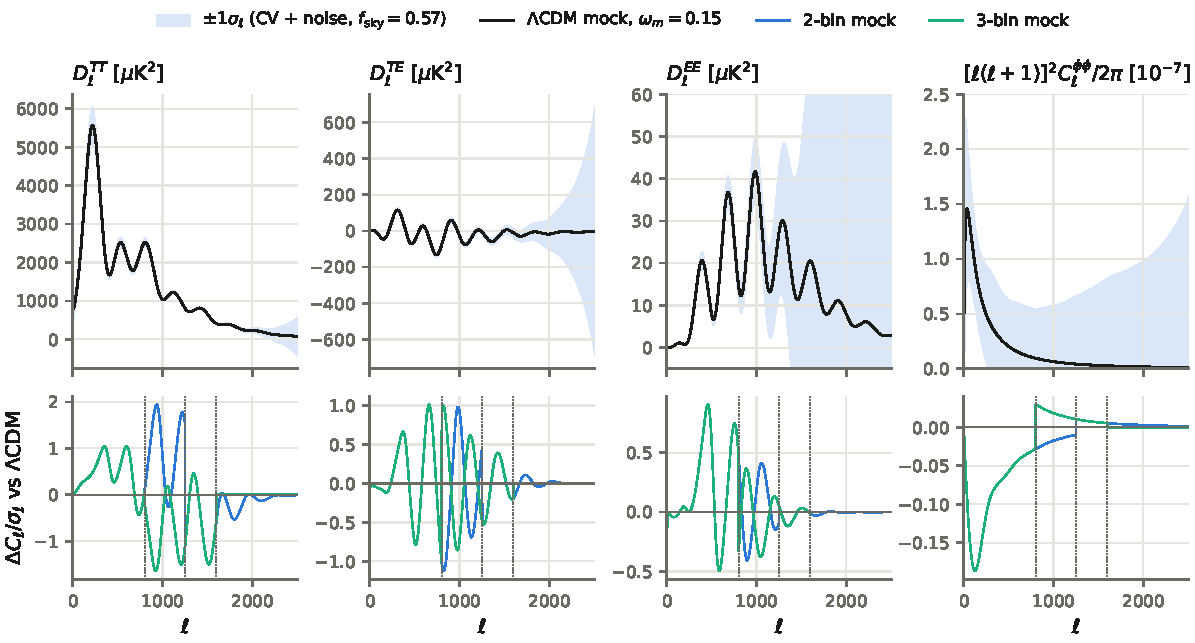
\includegraphics[width=0.8\textwidth]{fiducial_spectra}

\vspace{-0.2em}
\begin{itemize}\small
  \item Top: \lcdm\ mock with the per-$\ell$ $1\sigma$ of our likelihood (CV + noise); TT is noise dominated above $\ell\approx1500$.
  \item Bottom: binned mocks minus \lcdm, in units of $\sigma_\ell$: up to $2\sigma$ \emph{per multipole}, over hundreds of multipoles.
\end{itemize}
\end{frame}

% ======================================================================
\begin{frame}{Choice of binning: Fisher forecast}
\centering
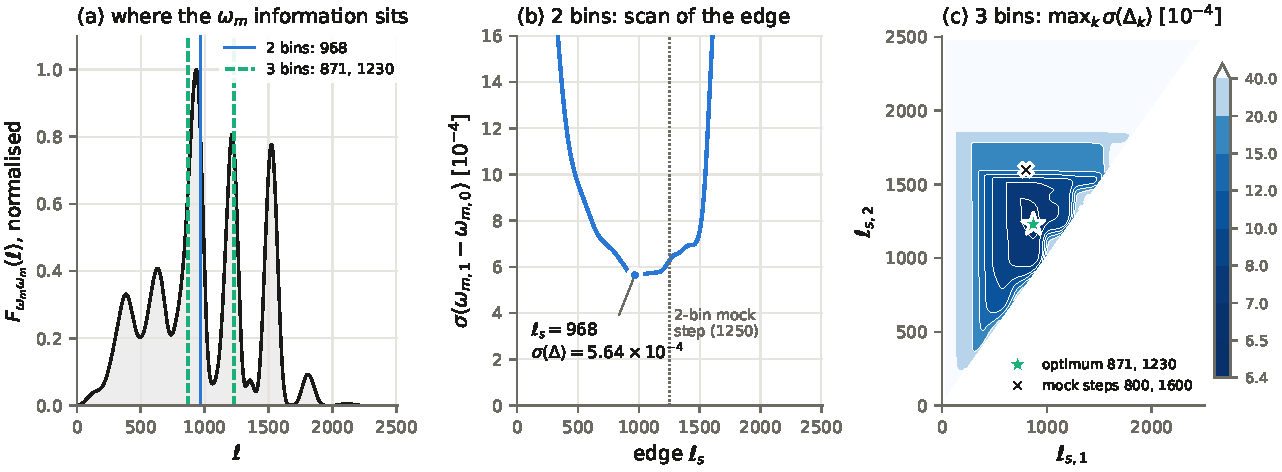
\includegraphics[width=0.8\textwidth]{binning_fisher}
\vspace{-0.3em}
\begin{columns}[T]
\column{0.5\textwidth}
\begin{itemize}\scriptsize
  \item Objective: minimise $\max_k \sigma(\omega_{m,k+1}-\omega_{m,k})$, marginalised over $\omega_b,h,\tau,n_s,A_s$ and the other bins.
  \item Fisher of this likelihood (TT, TE, EE + $d$), derivatives with real CLASS (5-point stencil; $<0.6\%$ change when steps are halved).
  \item Since $\partial C_\ell/\partial\omega_{m,i}=\partial C_\ell/\partial\omega_m\,\mathbb 1[\ell\in i]$, any binning is a cumulative sum $\Rightarrow$ exhaustive scans are cheap.
\end{itemize}
\column{0.48\textwidth}
\small
\begin{tabular}{@{}clll@{}}
\toprule
$N$ & edges & $\sigma(\omega_{m,i})\ [10^{-3}]$ & $\sigma(\Delta)\ [10^{-3}]$\\
\midrule
1 & --- & 1.21 & --- \\
2 & 968 & 1.22, 1.29 & 0.56 \\
3 & 871, 1230 & 1.22, 1.36, 1.39 & 0.65, 0.65 \\
\bottomrule
\end{tabular}

\vspace{0.3em}
{\scriptsize Optimum found by exhaustive scan ($N=2$), differential evolution with 3 seeds + brute force on a 5-$\ell$ grid ($N=3$): all agree.
Rounding to multiples of 25 costs $<0.1\%$.}
\end{columns}
\end{frame}

% ======================================================================
\begin{frame}{MCMC 1: \lcdm\ mock --- the null test}
\begin{columns}[T]
\column{0.56\textwidth}
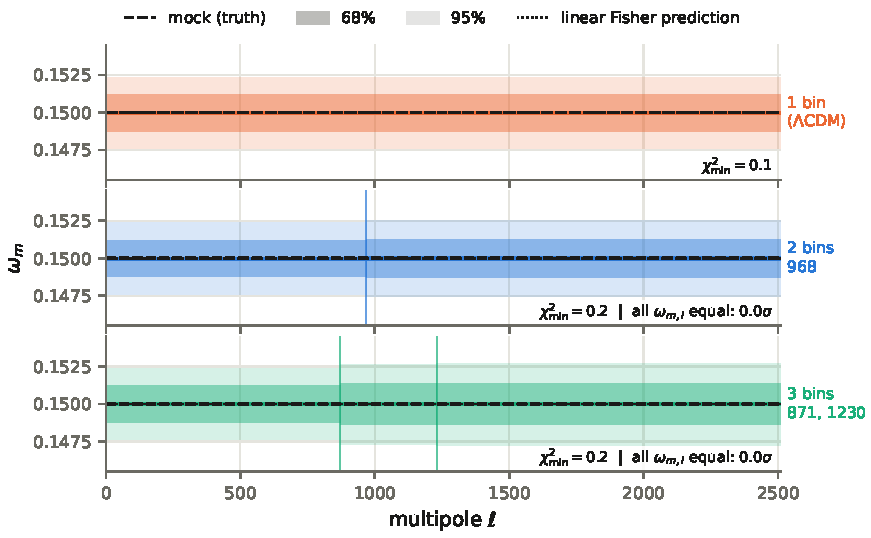
\includegraphics[width=\textwidth]{omega_ell_lcdm}
\column{0.42\textwidth}
\small
Fisher vs MCMC errors (\lcdm\ mock):

\vspace{0.2em}
{\scriptsize\setlength{\tabcolsep}{3pt}
\begin{tabular}{@{}lll@{}}
\toprule
& Fisher & MCMC \\
\midrule
1 bin: $\sigma(\om)$ & 1.21 & 1.21 \\
2 bins: $\sigma(\omega_{m,i})$ & 1.22, 1.29 & 1.22, 1.29 \\
\quad $\sigma(\Delta)$ & 0.56 & 0.56 \\
3 bins: $\sigma(\omega_{m,i})$ & 1.22, 1.36, 1.39 & 1.22, 1.37, 1.39 \\
\quad $\sigma(\Delta_k)$ & 0.65, 0.65 & 0.64, 0.64 \\
\bottomrule
\end{tabular}}
{\scriptsize\ (units of $10^{-3}$)}

\vspace{0.5em}
\begin{itemize}
  \item All bins recover $\om=0.150$; $\Delta$ consistent with 0 (test: $0.0\sigma$).
  \item $\chi^2_{\min}=0.1$--$0.2$ (noiseless mock).
  \item The other parameters do not care how many bins we free: next slide, top row.
\end{itemize}
\end{columns}
\end{frame}

% ======================================================================
\begin{frame}{MCMC 2: 2-bin mock, fitted with misplaced edges}
\begin{columns}[T]
\column{0.56\textwidth}
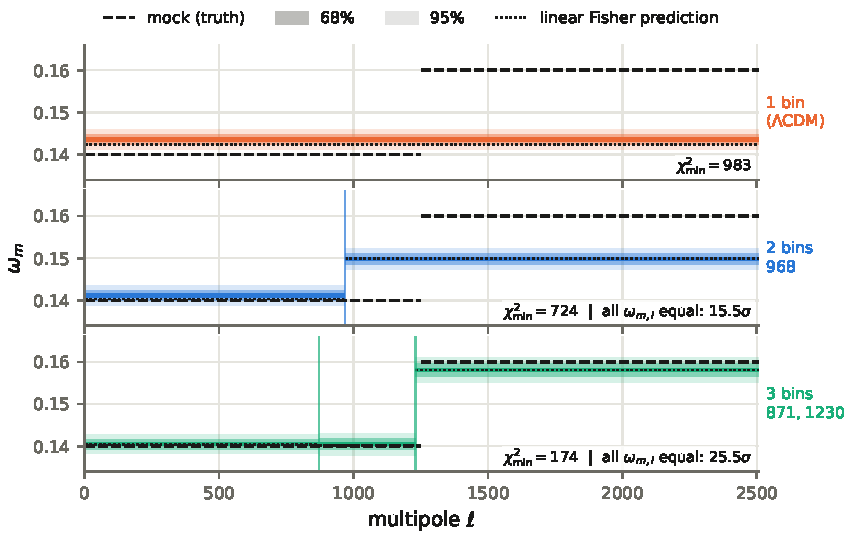
\includegraphics[width=\textwidth]{omega_ell_2bins}
\column{0.42\textwidth}
\small
Truth: step $0.14\to0.16$ at $\ell=1250$. Fitted edges: 968 (2 bins), 871 and 1230 (3 bins).
\begin{itemize}
  \item 2 bins: $\omega_{m,1}-\omega_{m,0}=0.0087\pm0.00056$ $\Rightarrow$ \lcdm\ rejected at $15.5\sigma$, although the edge is 280 multipoles off.
  \item 3 bins: the jump lands between bins 1 and 2 ($\Delta_{21}=0.0176\pm0.0007$); bins 0 and 1 agree. $25.5\sigma$.
  \item Bins that straddle the step return an information-weighted average: $0.1499$ for $\ell\in(968,2508]$.
  \item $\chi^2_{\min}$: $983\to724\to174$.
\end{itemize}
\takeaway{The binned model picks up the signal even when its edges do not match the truth.}
\end{columns}
\end{frame}

% ======================================================================
\begin{frame}{MCMC 3: 3-bin mock (0.14 $|$ 0.16 $|$ 0.15 at 800, 1600)}
\begin{columns}[T]
\column{0.56\textwidth}
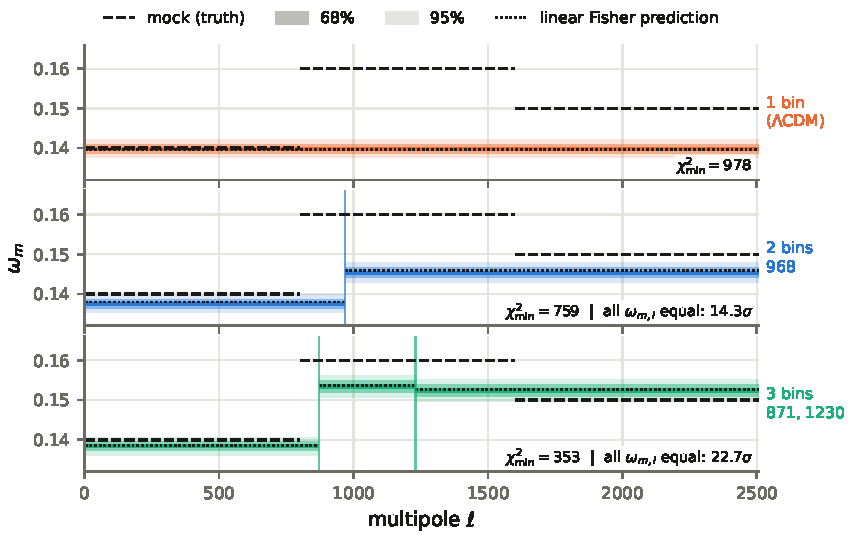
\includegraphics[width=\textwidth]{omega_ell_3bins}
\column{0.42\textwidth}
\small
\begin{itemize}
  \item 2 bins: $\Delta=0.0079\pm0.00055$, $14.3\sigma$.
  \item 3 bins: $\Delta_{10}=0.0151\pm0.0007$, $\Delta_{21}=-0.0011\pm0.0007$; \lcdm\ rejected at $22.7\sigma$.
  \item The rise at 800 is caught by the 871 edge; the small drop at 1600 (0.16$\to$0.15) falls inside the last bin and is averaged
  to 0.152.
  \item $\chi^2_{\min}$: $978\to759\to353$; with these edges the model cannot reach the truth, so $\chi^2_{\min}$ stays large.
\end{itemize}
\vspace{0.3em}
{\scriptsize Dotted lines: linear Fisher prediction of the best fit (slide~\ref{fr:linear}).}
\end{columns}
\end{frame}

% ======================================================================
\begin{frame}{\lcdm\ parameters: insensitive to extra bins, biased by a missed step}
\centering
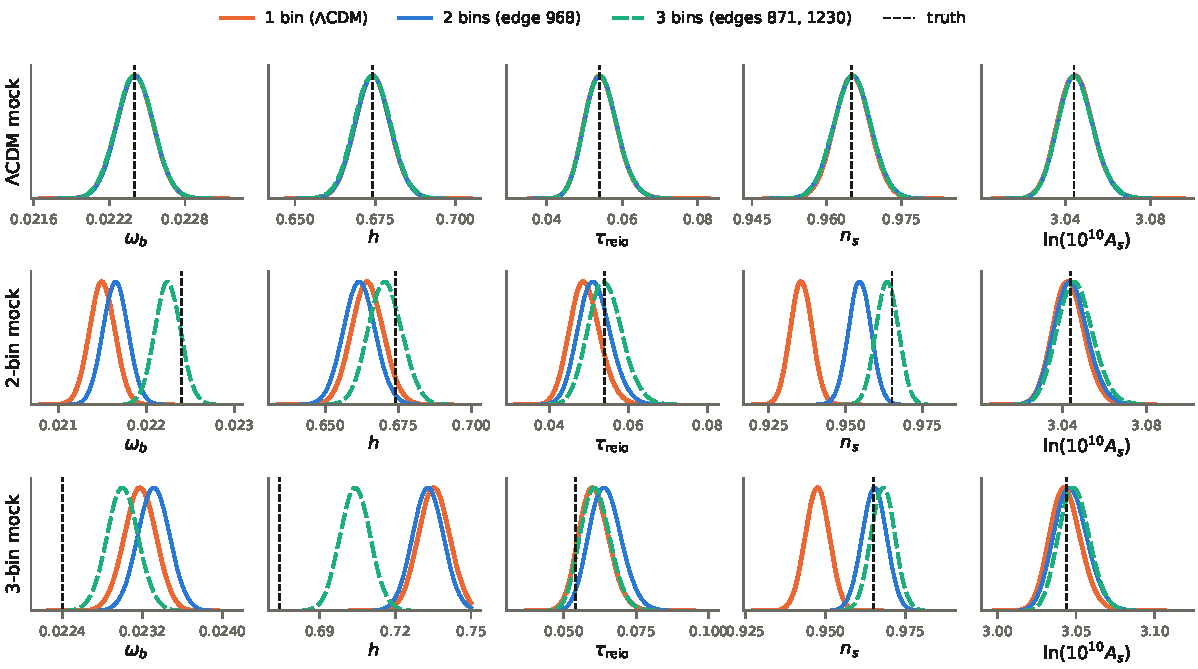
\includegraphics[width=0.8\textwidth]{theta_posteriors}
\vspace{-0.2em}
\begin{itemize}\scriptsize
  \item \lcdm\ mock (top): 1, 2 and 3 bins give the same posteriors (shifts $\le0.12\sigma$; $\sigma(h)$ 0.0055 $\to$ 0.0057). Freeing $\om$ per bin costs nothing.
  \item Binned mocks: the 1-bin (\lcdm) fit absorbs the step into $n_s$ ($-8.3\sigma$) and $\omega_b$ ($-6.3\sigma$), or into $h$ ($+10\sigma$,
  close to the prior edge 0.75). More bins remove most of the bias (2-bin mock, 3 bins: all $|{\rm shift}|\le1.1\sigma$).
\end{itemize}
\end{frame}

% ======================================================================
\begin{frame}{Bin posteriors and correlations}
\begin{columns}[T]
\column{0.42\textwidth}
\centering
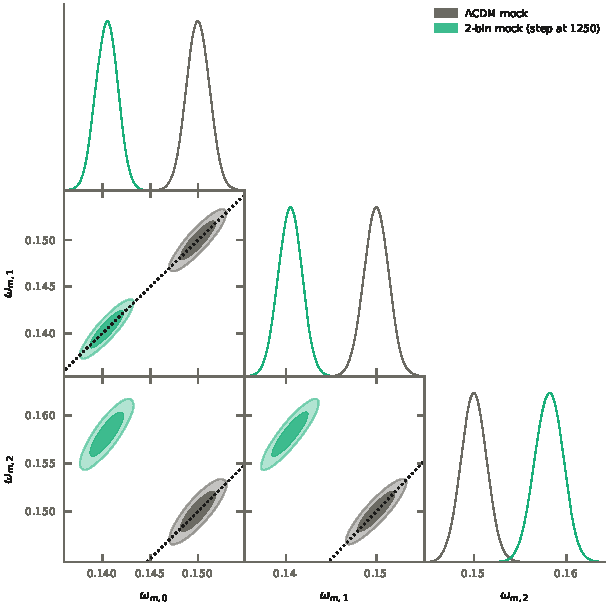
\includegraphics[width=0.95\textwidth]{omega_triangle}\\
{\scriptsize 3-bin fit. Dotted: $\omega_{m,i}=\omega_{m,j}$ (\lcdm).}
\column{0.56\textwidth}
\centering
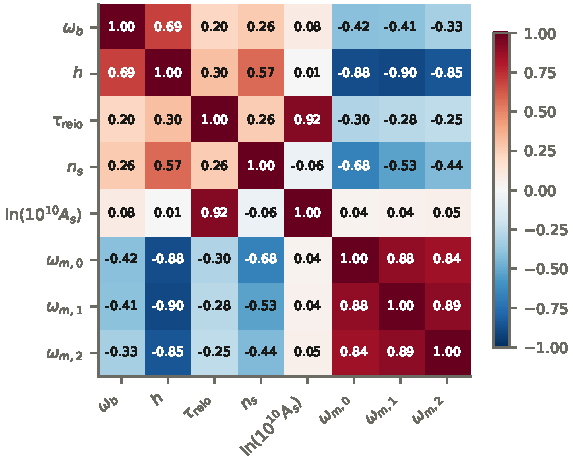
\includegraphics[width=0.66\textwidth]{correlation_3bins}\\
{\scriptsize Correlation matrix, 3-bin fit to the \lcdm\ mock.}
\vspace{0.3em}
\begin{itemize}\small
  \item Bins are strongly correlated with each other ($\rho=0.84$--$0.89$) and with $h$ ($\rho\approx-0.88$).
  \item The common mode goes into $h$; the differences are what the data pin down:
  $\sigma(\Delta)=0.56\times10^{-3}$ vs $\sigma(\omega_{m,i})=1.2$--$1.4\times10^{-3}$.
\end{itemize}
\end{columns}
\end{frame}

% ======================================================================
\begin{frame}{Comparison with the model: a linear Fisher prediction reproduces the chains}\label{fr:linear}
\begin{columns}[T]
\column{0.5\textwidth}
\small
Best fit of the binned model to a mock with $\om(\ell)$, to first order:
\[ \delta\hat p = F_{\rm fit}^{-1}\, b,\qquad b_a=\sum_\ell F_\ell^{\,a\,\om}\,\delta\om(\ell),\]
\[ \chi^2_{\min}=\sum_\ell F_\ell^{\,\om\om}\,\delta\om(\ell)^2-b^T F_{\rm fit}^{-1}b . \]

\vspace{0.2em}
\begin{tabular}{@{}llrr@{}}
\toprule
mock & fit & $\chi^2_{\min}$ linear & MCMC \\
\midrule
2-bin & 1 bin & 1010 & 983 \\
      & 2 bins & 726 & 724 \\
      & 3 bins & 164 & 174 \\
3-bin & 1 bin & 945 & 979 \\
      & 2 bins & 748 & 759 \\
      & 3 bins & 354 & 353 \\
\bottomrule
\end{tabular}
\column{0.48\textwidth}
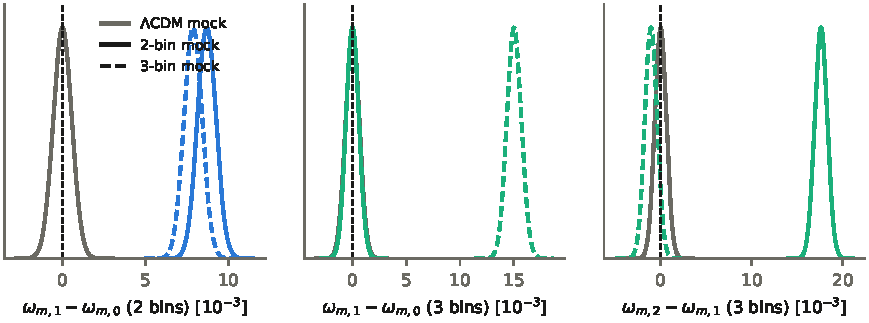
\includegraphics[width=\textwidth]{delta_posteriors}\\
{\scriptsize $\Delta$ posteriors. Colour = fitted binning (blue: 2 bins, green: 3 bins).}
\vspace{0.3em}
\begin{itemize}\small
  \item Bin values agree with MCMC to $\lesssim0.001$ (dotted lines on slides 8--9), \lcdm\ parameters to $\lesssim0.5\sigma$.
  \item The chains are understood: each fitted bin returns the Fisher-weighted mean of $\om(\ell)$ over its range,
  and the rest is absorbed by $n_s$, $\omega_b$, $h$.
\end{itemize}
\end{columns}
\end{frame}

% ======================================================================
\begin{frame}{Derivatives and the discontinuity at the edges}\label{fr:edges}
\begin{columns}[T]
\column{0.47\textwidth}
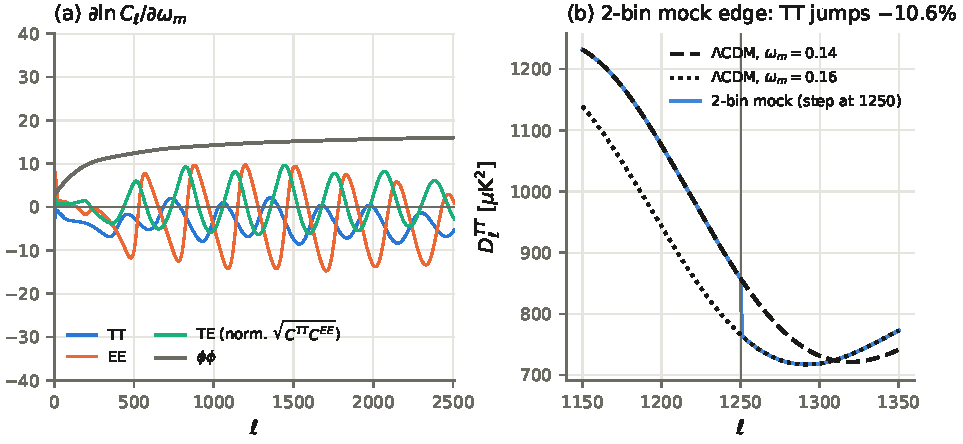
\includegraphics[width=\textwidth]{edges_derivatives}
\column{0.51\textwidth}
\tiny
Jump in $C_\ell$ across an edge (real CLASS) and the error it puts in a central-difference $\partial C_\ell/\partial\ell$ at the edge:

\vspace{0.2em}
\setlength{\tabcolsep}{3pt}
\begin{tabular}{@{}lrrrr@{}}
\toprule
& TT & EE & TE$^\dagger$ & $\phi\phi$ \\
\midrule
\multicolumn{5}{@{}l}{$1\sigma(\Delta)$ step ($5.6\times10^{-4}$) at 1250} \\
\quad jump & $-0.31\%$ & $+0.24\%$ & $-0.29\%$ & $+0.8\%$ \\
\quad natural $\ell\to\ell+1$ & $-0.54\%$ & $+0.33\%$ & $-0.35\%$ & $-0.5\%$ \\
\quad err.\ on $\partial C/\partial\ell$ & $+28\%$ & $+35\%$ & $+42\%$ & $-88\%$ \\
\midrule
\multicolumn{5}{@{}l}{mock step $0.14\to0.16$ at 1250} \\
\quad jump & $-10.6\%$ & $+9.0\%$ & $-10.2\%$ & $+35\%$ \\
\quad err.\ on $\partial C/\partial\ell$ & $\times 9$ & $\times 9$ & $\times 19$ & $\times 36$ \\
\bottomrule
\end{tabular}

{$^\dagger$TE relative to $\sqrt{C^{TT}C^{EE}}$. Same size at 871, 968, 1230.}
\end{columns}
\vspace{0.4em}
\begin{itemize}\small
  \item $|\partial\ln C_\ell/\partial\om|\sim5$--$15$, so a step $\delta\om$ makes a jump $\approx\partial\ln C/\partial\om\cdot\delta\om$; at a just-detectable step it is about half the normal change between neighbouring multipoles.
  \item Our likelihood and the Fisher use $C_\ell$ at fixed $\ell$ (and $\partial/\partial\theta$ only) $\Rightarrow$ unaffected. Plik, CamSpec, Commander and Planck lensing never take $\partial C_\ell/\partial\ell$;
  SPT-3G (aberration, super-sample lensing) and Cobaya's CMBlikes aberration do $\Rightarrow$ put edges on bandpower edges there.
\end{itemize}
\end{frame}

% ======================================================================
\begin{frame}{Benchmark 1: spectra, CLASS vs CosmoPower}
\centering
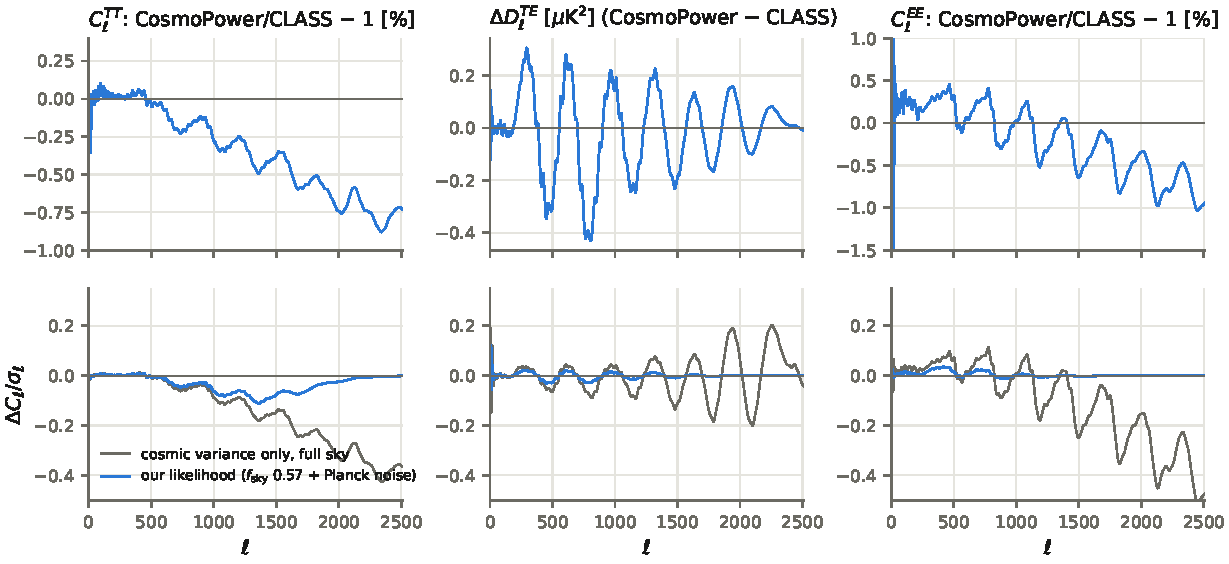
\includegraphics[width=0.8\textwidth]{bench_spectra}
\vspace{-0.3em}
\begin{columns}[T]
\column{0.5\textwidth}
\begin{itemize}\scriptsize
  \item At the mock point ($\om=0.15$): CosmoPower is low in the damping tail, TT $-0.3\%$ at $\ell=1000$, $-0.7\%$ at 2000--2500; EE up to $-1\%$.
  \item Per multipole in our likelihood: $\le0.11\sigma_\ell$ (TT), $\le0.04\sigma_\ell$ (TE, EE). Cosmic-variance-limited: up to $0.4$--$0.5\sigma$.
\end{itemize}
\column{0.48\textwidth}
\begin{itemize}\scriptsize
  \item Not CLASS settings: \texttt{cl\_ref.pre} changes CLASS by $\le0.08\%$; CAMB (massless $\nu$, linear lensing) shows the same gap.
  The emulators were trained on CAMB over a very wide box; the size matches the CosmoPower paper's full-box accuracy ($\sim0.2\sigma_{\rm CMB}$, App.~C).
  \item $\ell$ indexing checked: best-fit shift $|d|\le0.27$; an injected 1-multipole shift is recovered.
\end{itemize}
\end{columns}
\end{frame}

% ======================================================================
\begin{frame}{Benchmark 2: MCMC level}
\begin{columns}[T]
\column{0.46\textwidth}
\centering
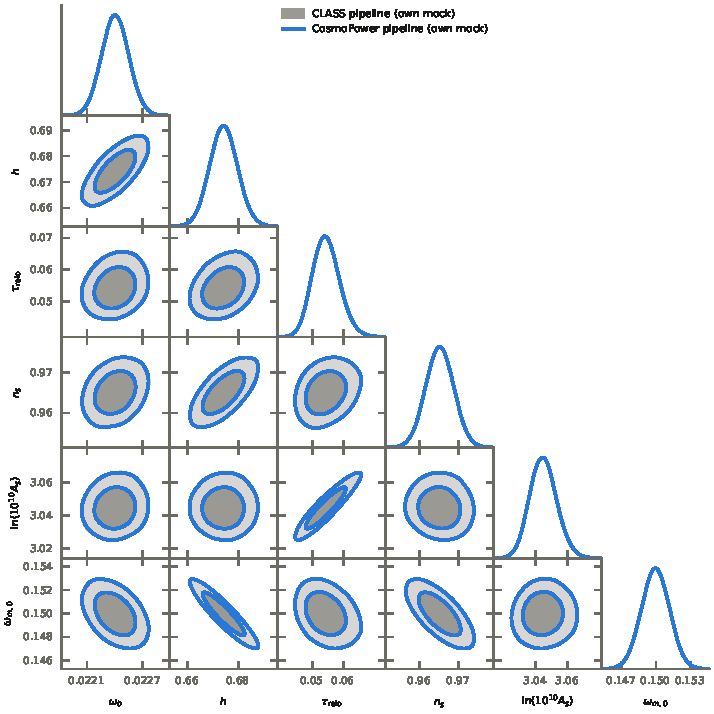
\includegraphics[width=0.98\textwidth]{bench_posteriors}\\
{\scriptsize \lcdm\ mock, 1 bin. Each pipeline fits its own mock.}
\column{0.52\textwidth}
\small
{\bfseries Same pipeline, different spectra code} (each with its own mock):
posteriors identical; mean shifts $\le0.02\sigma$, error ratios 0.98--1.00.

\vspace{0.3em}
{\bfseries Cross test} (forecast): CosmoPower model fitted to a CLASS mock --- what real data would see.
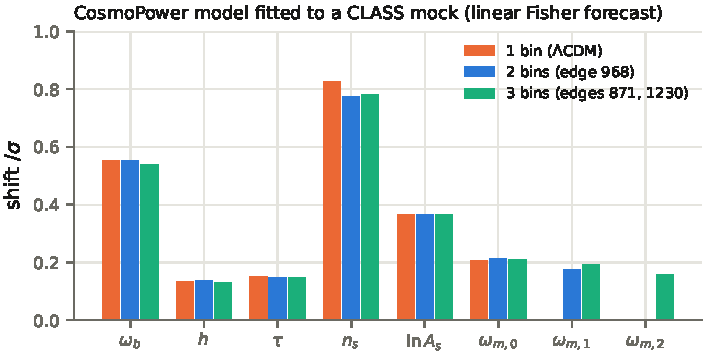
\includegraphics[width=\textwidth]{bench_bias}
\begin{itemize}\scriptsize
  \item Emulator error is absorbed by $n_s$ ($+0.8\sigma$), $\omega_b$ ($+0.55\sigma$), $A_s$ ($+0.37\sigma$); $\chi^2$ 6.4 $\to$ 0.5 after refit.
  \item Spurious $\Delta\omega_m$ between bins: $\le0.06\sigma$. (Supersedes our earlier single-parameter estimate of $+0.001$.)
\end{itemize}
\end{columns}
\end{frame}

% ======================================================================
\begin{frame}{Summary and next steps}
\begin{columns}[T]
\column{0.5\textwidth}
{\bfseries Where we are}
\begin{itemize}\small
  \item Binned-$\om$ model in MontePython with two interchangeable back-ends; mock Planck-like likelihood (TT, TE, EE + lensing).
  \item Fisher-optimal edges: 968 (2 bins); 871, 1230 (3 bins). $\sigma(\Delta)=0.56$--$0.65\times10^{-3}$, confirmed by MCMC.
  \item Freeing $\om$ per bin leaves the \lcdm\ posteriors unchanged on a \lcdm\ mock.
  \item Misplaced bins still detect injected steps at 14--26$\sigma$; a \lcdm\ fit instead hides them in $n_s$, $\omega_b$, $h$.
  \item The chains match a linear Fisher prediction.
  \item CosmoPower vs CLASS: identical posteriors on their own mocks; forecast emulator bias on real data is in the \lcdm\ parameters ($\le0.8\sigma$),
  not in $\Delta\om$.
\end{itemize}
\column{0.48\textwidth}
{\bfseries Next}
\begin{itemize}\small
  \item Cross-pipeline MCMC: CosmoPower chains on the CLASS mock (check the forecast bias).
  \item CLASS counterparts of the binned runs (same folders).
  \item Sensitivity: smallest detectable step vs its position; more bins (4--10).
  \item Real data: Planck likelihoods via clik with CLASS (or a narrow-box emulator retrained on CLASS); edges on bandpower edges.
\end{itemize}
\end{columns}
\end{frame}

% ======================================================================
\appendix
\begin{frame}[plain]
  \vfill\centering{\color{muted}\Large Backup}\vfill
\end{frame}

\begin{frame}{Backup: convergence and best fits (CosmoPower pipeline)}
\centering\small
\begin{tabular}{@{}llcccl@{}}
\toprule
mock & fit & acceptance & max $R-1$ & $\chi^2_{\min}$ & \lcdm\ test \\
\midrule
\lcdm & 1 bin & 0.25 & 0.0002 & 0.09 & --- \\
      & 2 bins & 0.25 & 0.0007 & 0.17 & $0.0\sigma$ \\
      & 3 bins & 0.14 & 0.0015 & 0.17 & $0.0\sigma$ \\
\midrule
2-bin & 1 bin & 0.25 & 0.0004 & 983.0 & --- \\
      & 2 bins & 0.24 & 0.0007 & 724.1 & $15.5\sigma$ \\
      & 3 bins & 0.14 & 0.0013 & 173.5 & $25.5\sigma$ \\
\midrule
3-bin & 1 bin & 0.30 & 0.0006 & 978.5 & --- \\
      & 2 bins & 0.26 & 0.0008 & 759.5 & $14.3\sigma$ \\
      & 3 bins & 0.15 & 0.0016 & 353.0 & $22.7\sigma$ \\
\midrule
\multicolumn{2}{@{}l}{CLASS pipeline, \lcdm\ mock, 1 bin} & 0.26 & --- & 0.08 & --- \\
\bottomrule
\end{tabular}

\vspace{0.6em}
{\scriptsize 8 chains $\times10^5$ steps each, 30\% burn-in; $R-1$: multiplicity-weighted Gelman--Rubin per parameter, worst parameter shown.
\lcdm\ test: Gaussian $\chi^2$ of $(\Delta_1,\dots,\Delta_{N-1})$ against 0, converted to a two-sided significance.}
\end{frame}

\begin{frame}{Backup: marginal constraints, all runs}
\centering\scriptsize
\setlength{\tabcolsep}{4pt}
\begin{tabular}{@{}llccccccc@{}}
\toprule
mock & fit & $10^2\omega_b$ & $h$ & $\tau$ & $n_s$ & $\ln10^{10}A_s$ & $\omega_{m,i}$ \\
\midrule
truth & & 2.240 & 0.674 & 0.054 & 0.965 & 3.044 & \\
\midrule
\lcdm & 1 & 2.240(15) & 0.6742(55) & 0.0545(44) & 0.9651(36) & 3.045(8) & 0.1500(12) \\
      & 2 & 2.241(15) & 0.6742(55) & 0.0545(43) & 0.9651(37) & 3.045(8) & 0.1500, 0.1500 \\
      & 3 & 2.240(15) & 0.6741(57) & 0.0545(44) & 0.9651(37) & 3.045(8) & 0.1500, 0.1500, 0.1500 \\
\midrule
2-bin & 1 & 2.150(14) & 0.6645(55) & 0.0491(38) & 0.9356(35) & 3.043(8) & 0.1436(12) \\
      & 2 & 2.165(14) & 0.6616(55) & 0.0515(41) & 0.9545(37) & 3.044(8) & 0.1412, 0.1499 \\
      & 3 & 2.224(15) & 0.6705(57) & 0.0543(44) & 0.9635(36) & 3.046(9) & 0.1405, 0.1405, 0.1581 \\
\midrule
3-bin & 1 & 2.318(16) & 0.7352(61) & 0.0606(52) & 0.9474(37) & 3.043(10) & 0.1399(12) \\
      & 2 & 2.331(16) & 0.7329(61) & 0.0645(56) & 0.9652(38) & 3.047(11) & 0.1375, 0.1453 \\
      & 3 & 2.300(16) & 0.7041(60) & 0.0610(51) & 0.9679(37) & 3.049(10) & 0.1384, 0.1534, 0.1524 \\
\bottomrule
\end{tabular}

\vspace{0.5em}
{\scriptsize Mean (error on the last digits). $\sigma(\omega_{m,i})$: 1.2--1.5$\times10^{-3}$, see slide on errors.
Binnings: 2 bins = edge 968; 3 bins = edges 871, 1230. 3-bin mock, 1--2 bins: $h$ is within $3\sigma$ of the prior edge 0.75.}
\end{frame}

\begin{frame}{Backup: what the emulator error is, and is not}
\centering\scriptsize
Emulator / reference $-1$ [\%], TT unless noted, at $\omega_b=0.0224$, $\omega_{\rm cdm}=0.12$, $h=0.674$, $\tau=0.054$, $n_s=0.965$, $\ln10^{10}A_s=3.044$:

\vspace{0.3em}
\begin{tabular}{@{}lrrrrrr@{}}
\toprule
reference & $\ell=30$ & 500 & 1000 & 1500 & 2000 & 2500 \\
\midrule
CLASS 3.4, massless $\nu$, linear lensing & $+0.03$ & $-0.02$ & $-0.22$ & $-0.34$ & $-0.71$ & $-0.78$ \\
\quad EE & $+0.46$ & $+0.23$ & $-0.02$ & $-0.61$ & $-0.28$ & $-0.95$ \\
CLASS 3.4, $m_\nu=0.06$ eV & $+0.01$ & $-0.26$ & $+0.15$ & $+0.53$ & $-0.70$ & $+0.41$ \\
CLASS 3.4, halofit lensing & $+0.03$ & $-0.01$ & $-0.22$ & $-0.27$ & $-0.91$ & $-1.77$ \\
CLASS 2.9.4, massless $\nu$, linear & $+0.03$ & $+0.00$ & $-0.20$ & $-0.31$ & $-0.55$ & $-0.52$ \\
CAMB 2.0.4, $m_\nu=0$, linear lensing & $+0.05$ & $-0.10$ & $-0.19$ & $-0.31$ & $-0.64$ & $-0.56$ \\
CAMB 2.0.4, $m_\nu=0$, nonlinear lensing & $+0.04$ & $-0.08$ & $-0.19$ & $-0.23$ & $-0.82$ & $-1.49$ \\
\midrule
CLASS default vs \texttt{cl\_ref.pre} (precision) & $+0.02$ & $-0.08$ & $-0.05$ & $-0.03$ & $-0.05$ & $-0.04$ \\
\bottomrule
\end{tabular}

\vspace{0.5em}
\begin{itemize}\scriptsize
  \item Massive $\nu$ gives oscillating residuals (peak shift); nonlinear lensing makes the tail worse $\Rightarrow$ emulator = massless $\nu$ + linear lensing.
  \item CosmoPower paper metric ($|\Delta C|/\sigma_{\rm CMB}$, $f_{\rm sky}=0.4$, SO goal noise): TT $0.15$--$0.19\sigma$ above $\ell\approx1600$;
  paper: 99\% $<0.1\sigma$ in a $5\sigma$-Planck box, $\sim0.2\sigma$ over the full training box.
\end{itemize}
\end{frame}

\begin{frame}{Backup: marginalising the Fisher over the \lcdm\ parameters}
\small
With $x=\delta\om$, $y=\delta\theta$ ($\theta=\omega_b,h,\tau,n_s,A_s$) and
$F=\begin{pmatrix} a & b^T\\ b & A\end{pmatrix}$:
\[
P(x)\propto\int d^5y\,\exp\!\Big[-\tfrac12\big(a x^2+2x\,b^Ty+y^TAy\big)\Big]
\propto\exp\!\Big[-\tfrac12 x^2\big(a-b^TA^{-1}b\big)\Big],
\]
so $\sigma^2(\om)=(a-b^TA^{-1}b)^{-1}=(F^{-1})_{\om\om}$ (Schur complement).

\vspace{0.6em}
For $N$ bins the same algebra with $a\to\mathrm{diag}(F^{\om\om}_{(i)})$ and $b\to B_{ai}=\sum_{\ell\in i}F_\ell^{\,a\,\om}$ gives the
bin covariance
\[ C_{\om}=\big[\mathrm{diag}(F^{\om\om}_{(i)})-B^TA^{-1}B\big]^{-1},\qquad
\sigma^2(\Delta_k)=C_{kk}+C_{k+1,k+1}-2C_{k,k+1}. \]
All per-bin sums come from cumulative sums of the per-$\ell$ Fisher blocks, so a binning costs microseconds.

\vspace{0.6em}
{\scriptsize Edge rounding (best edges on a grid): $N=2$: 970 / 975 / 950 for steps 10 / 25 / 50, $+0.0\%$ / $+0.0\%$ / $+0.3\%$ in $\sigma(\Delta)$.
$N=3$: (870, 1230) / (875, 1225) / (850, 1250): $+0.1\%$ / $+0.1\%$ / $+1.0\%$. Equal-information edges (943; 831, 1188) cost $+1\%$ / $+7\%$.}
\end{frame}

\end{document}
